\section{Simulations}

\subsection{Numerical implementation}

\subsubsection{Evolution equation}

Starting from \autoref{eq:eq1}, we want to obtain an equation to numerically calculate the wave height at the next timestep \(t_{i+1}\) using the previous heights at positions \(x_i\), \(x_{i-1}\) and \(x_{i+1}\). Using the following approximations for the derivatives
\begin{equation}
    \frac{\partial F}{\partial x}(x_i) \approx \frac{F(x_{i+1}) - F(x_{i-1})}{2 \Delta x}
    , \qquad
    \frac{\partial^2 F}{\partial x^2}(x_i) \approx \frac{F(x_{i+1}) - 2 F(x_i) + F(x_{i-1})}{(\Delta x)^2}
\end{equation}
where \(F\) is a generic function representing either \(f\) or \(h_0\), \(\Delta x = x_{i+1} - x_i\) and \(x\) is a generic variable representing either \(x\) or \(t\). \autoref{eq:eq1} is equivalent to:
\begin{equation}
    \frac{\partial^2 f}{\partial t^2} = g \frac{\partial h_0}{\partial x} \frac{\partial f}{\partial x} + g h_0 \frac{\partial^2 f}{\partial x^2}
\end{equation}
Then using the previously mentioned formulas:
\begin{equation}
    \begin{aligned}
        \frac{f(x_i, t_{i+1}) - 2 f(x_i, t_i) + f(x_i, t_{i-1})}{(\Delta t)^2} &= g \left( \frac{h_0(x_{i+1}) - h_0(x_{i-1})}{2 \Delta x} \right) \left( \frac{f(x_{i+1}, t_i) - f(x_{i-1}, t_i)}{2 \Delta x} \right) \\
        &+ g h_0(x_i) \frac{f(x_{i+1}, t_i) - 2 f(x_i, t_i) + f(x_{i-1}, t_i)}{(\Delta x)^2}
    \end{aligned}
\end{equation}
By rearanging and identifying the Courant-Friedrichs-Lewy constant \(\beta(x) = u(x) \frac{\Delta t}{\Delta x} = \sqrt{g h_0(x)} \frac{\Delta t}{\Delta x}\) we get the following equation:
\begin{equation}
    \begin{aligned}
        f(x_i, t_{i+1}) &= \frac{g}{4} \left( \beta(x_{i+1})^2 - \beta(x_{i-1})^2 \right) \left( f(x_{i+1}, t_i) - f(x_{i-1}, t_i) \right) \\
        &+ \beta(x_i)^2 (f(x_{i+1}, t_i) - 2 f(x_i, t_i) + f(x_{i-1}, t_i)) \\
        &+ f(x_i,t_i) \\
        &- f(x_i,t_{i-1})
    \end{aligned}
\end{equation}
The evolution for \autoref{eq:eq2} is taken from \cite{physnumbook}, equation 4.43.

\subsubsection{Border conditions}

The simulation implements border conditions for a fixed border (wave has a specific height at border), a free border (the wave is allowed to move as it pleases along the border) and an exit condition (the wave continues as if there was no border). These conditions are given in a Numerical Physics book \cite{physnumbook} (section 4.2.1), for the left and right borders. We will derive the exit conditions for the left border here. Under this condition, the left border only has a retrograde wave, i.e. \(f(x, t) = G(x + |u| t)\) TODO: NOTATION, VOIR PARTIE THEORIE. Differentiating w.r.t. to \(t\) and \(x\), at \(x = x_L\) (left border) we obtain the following relationship:
\begin{gather}
    \frac{\partial f}{\partial t}(x_L, t) = \frac{\partial G(x_L + |u| t)}{\partial t} = |u| G'(x_L - |u| t) \\
    \frac{\partial f}{\partial x}(x_L, t) = G'(x_L + |u| t) \\
    \implies \frac{\partial f}{\partial t}(x_L, t) = |u| \frac{\partial f}{\partial x}(x_L, t)
\end{gather}
Discretising using the "forward" finite difference method, i.e. \(F(x_i) \approx (F(x_{i+1}) - F(x_i))/\Delta x\), for both time and space derivatives, and identifying \(x_L \equiv x_0\), we get:
\begin{equation}
    \frac{f(x_0,t_{n+1}) - f(x_0, t_n)}{\Delta t} = |u| \frac{f(x_1, t_n) - f(x_0, t_n)}{\Delta x}
\end{equation}
Rearanging and identifying the CFL constant we then get:
\begin{equation}
    f(x_0, t_{n+1}) = f(x_0, t_n) + \beta \left( f(x_1, t_n) - f(x_0, t_n) \right)
\end{equation}

\subsubsection{Initial conditions}

The initial conditions for a left and right moving wave, as well as a static wave were implemented using equations 4.48 to 4.50 given in \cite{physnumbook}.

\subsection{Smol basin for smol duckies}

% feur

\subsection{Oceanic wave on a coral reef}

In this section we will use the following function for oceanic depth:
\begin{equation}
    h_0(x) = \begin{cases}
        \begin{aligned}
            &\scriptstyle{h_L} &&\scriptstyle{(x_L \le x \le x_a)} \\
            &\scriptstyle{\frac{1}{2}(h_L + h_C) + \frac{1}{2}(h_L - h_C) \cos \left( \pi \frac{x-x_a}{x_b-x_a} \right)} &&\scriptstyle{(x_a < x < x_b)} \\
            &\scriptstyle{h_C} &&\scriptstyle{(x_b \le x \le x_c)} \\
            &\scriptstyle{\frac{1}{2}(h_R + h_C) - \frac{1}{2}(h_R - h_C) \cos \left( \pi \frac{x-x_c}{x_d-x_c} \right)} &&\scriptstyle{(x_c < x < x_d)} \\
            &\scriptstyle{h_R} &&\scriptstyle{(x_d \le x \le x_R)}
        \end{aligned}
    \end{cases}
\end{equation}
We will choose \(h_L = 7000\)m, \(h_C = 35\)m, \(h_R = 200\)m, \(x_L = 0\)m, \(x_a = 300\)km, \(x_b = 700\)km, \(x_c = 720\)km, \(x_d = 850\)km and \(x_R = 1000\)km. The initial conditions will be a right moving wave with \(x_1 = 50\)km, \(x_2 = 250\)km and amplitude \(A = 1\)m. Both border conditions will be set to exit, to be more representative of an actual large ocean. The simulations were done until the wave passes the coral reef entierely, which corresponds to a time of about \(t = 12000\). The timestep \(\Delta t\) was chosen such that \(\max(\beta_{\textrm{CFL}}) = 1\), which is \(\Delta t = \Delta x / \max_x(u(x)^2)\). The number of intervals was chosen to be 8192.

\autoref{fig:corail_eq1_mouv} shows the obtained wave motion when using \autoref{eq:eq1}. We can see that around \(x=600\)km, the wave slows down considerably with a peak in amplitude, which corresponds to when the wave is right above the reef. We will study the amplitude and speed later. The observed behavior makes sense intuitively, as a wave would indeed get larger when the water becomes less deep.

\begin{figure}[h]
    \centering
    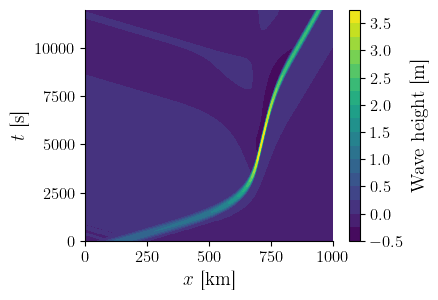
\includegraphics[width=0.6\linewidth]{figures/corail_eq1_mouvement_vague.png}
    \caption{Wave amplitude as a function of space and time. Simulated using \(n=8192\) intervals, until \(t=12000\)}
    \label{fig:corail_eq1_mouv}
\end{figure}

The maximum amplitude of the wave was obtained using a quadratic fit for every point around the time of its maximum amplitude. The maximum of the fit gave the maximum amplitude. Results are shown in \autoref{fig:corail_eq1_amplitude}. The simulation shows that the maximum amplitude increase up to the point of the coral reef, remains more or less constant on top of the reef and then goes back down. The peak amplitude above the reef (\(x_b < x < x_c\)) was found to be about 3.58m, while after the reef (\(x_d<x<x_R\)) the maximum amplitude was 2.30m. When compared to the WKB solution on \autoref{eq:eq2}, we can see that the phenomenon is completely inverted: for WKB, the amplitude lessens above the reef and increases back again after. This discrepency could be attributed to higher order terms in the expansion.

Using the analysis done on the amplitude, the speed of the peak of the wave was calculated using the time \(t_{\textrm{peak},i}\) at which the fitted function is maximal. Then for every point \(x_i\), except for border cases, the speed is given by \(v_i = (x_{i+k} - x_{i-k})/(t_{\textrm{peak},i+k} - t_{\textrm{peak},i-k})\), where \(k\) is chosen such that the oscillations in \(v\) are minimal. The results are shown in \autoref{fig:corail_eq1_vitesse}. We can see that the speed decrease drastically between the starting position of the wave and the coral reef, by a factor of about 11: the speed above the reef was found to be 18 m/s, while the initial speed was 261 m/s. After the reef, the speed increases again to around 42 m/s. The simulation matches the WKB solution exactly. This is because when analysing both \autoref{eq:eq1} and \autoref{eq:eq2} using WKB, we find the same result for the speed \(u(x) = \sqrt{gh_0(x)}\). MARTIN VERIFIE STP J'AI PAS TOUT COMPRIS

\begin{figure}[h]
    \centering
    \begin{subfigure}{0.48\linewidth}
        \centering
        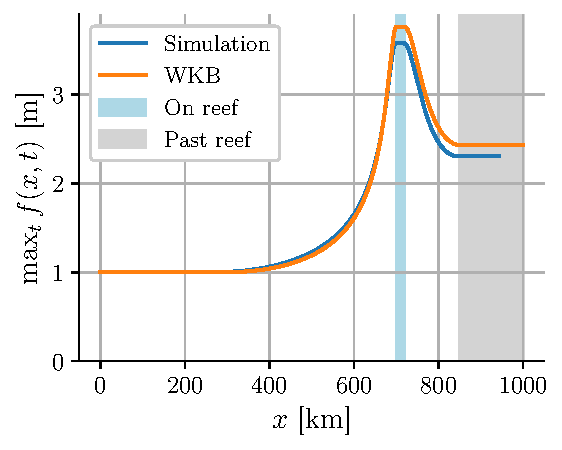
\includegraphics[width=\linewidth]{figures/corail_eq1_amplitude_wkb.pdf}
        \caption{Maximum amplitude reached at each position}
        \label{fig:corail_eq1_amplitude}
    \end{subfigure}
    \begin{subfigure}{0.48\linewidth}
        \centering
        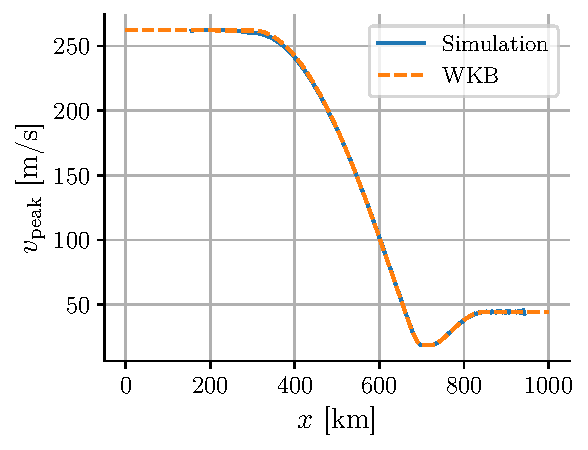
\includegraphics[width=\linewidth]{figures/corail_eq1_vitesse_wkb.pdf}
        \caption{Speed of wave peak}
        \label{fig:corail_eq1_vitesse}
    \end{subfigure}
    \caption{Properties of the wave going towards the coral reef, compared to WKB solution. Simulated using \(n=8192\) intervals, until \(t=12000\)}
    \label{fig:corail_eq1_properties}
\end{figure}

FEUR PARTIE (D)

Let's now analyse what happens when we simulate the system using the wrong although maybe intuitively plausible equation, \autoref{eq:eq2}. The resulting wave can be seen in \autoref{fig:corail_eq2_mouvement}. While the result looks similar at a glance to the result at the begining of this section, we can see that the amplitude of the wave decreases above the reef! Analysing this further using the same methods as described previously, we obtain a plot of the maximal amplitude and speed of the wave peak shown in \autoref{fig:corail_eq2_amplitude}. This time, the results match the WKB solution almost exactly for the amplitude and exactly for the speed. While the results are not realistic physically, it remains coherent that the WKB solution matches these simulations, because they were done using the same base equation.

\begin{figure}[h]
    \centering
    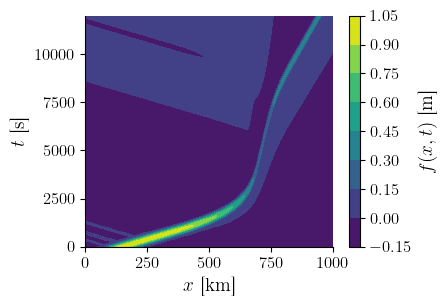
\includegraphics[width=0.6\linewidth]{figures/corail_eq2_mouvement_vague.png}
    \caption{Wave amplitude as a function of space and time, simulated following \autoref{eq:eq2}. Simulated with \(n=16328\) intervals until \(t=12000\)}
    \label{fig:corail_eq2_mouvement}
\end{figure}

\begin{figure}[h]
    \centering
    \begin{subfigure}{0.48\linewidth}
        \centering
        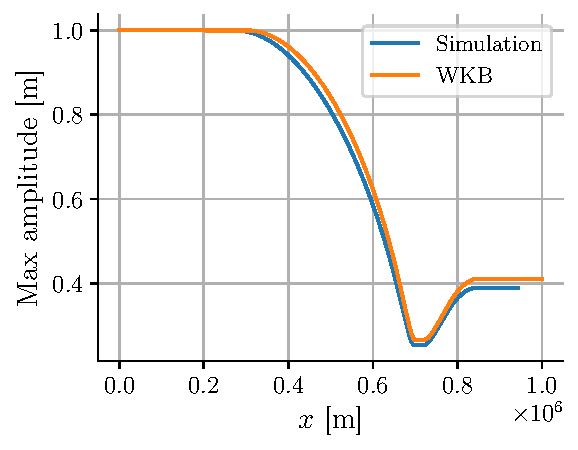
\includegraphics[width=\linewidth]{figures/corail_eq2_amplitude_wkb.pdf}
        \caption{Maximum amplitude reached at each position}
        \label{fig:corail_eq2_amplitude}
    \end{subfigure}
    \begin{subfigure}{0.48\linewidth}
        \centering
        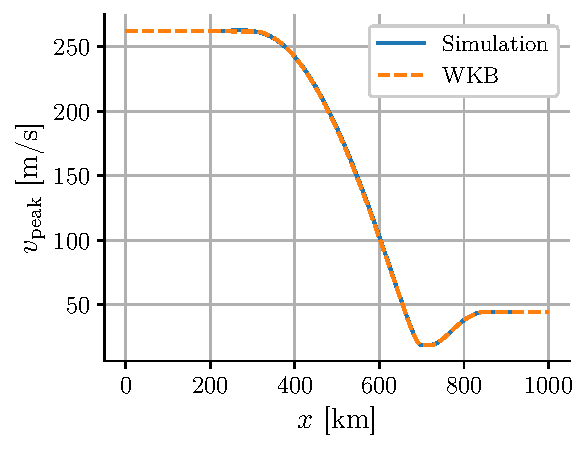
\includegraphics[width=\linewidth]{figures/corail_eq2_vitesse_wkb.pdf}
        \caption{Speed of wave peak}
        \label{fig:corail_eq2_vitesse}
    \end{subfigure}
    \caption{Properties of the wave going towards the coral reef, compared to WKB solution. Simulated w.r.t. \autoref{eq:eq2}, using \(n=8192\) intervals, until \(t=12000\)}
    \label{fig:corail_eq2_properties}
\end{figure}